\chapter{Analysis}

\dictum[Leslie Poles Hartley -- British writer]
{\flushright{}The past is a foreign country, they do things differently there.}

This chapter is dedicated to the analysis of the application domain. Outcomes of a
thorough investigation of the related constructs and principles are the main
content of the chapter. The first section explains the relationship between
actions, interactions and events. In section two the focus lies on the
detection of problems during the course of the game. After that, section three
leads to the learners' support. The last section of this chapter is about
pedagogical agents, a very promising technology in educational software, which have been
introduced earlier in this work (see chapter \ref{proposed_system_chapter}: Proposed System).

\section{Actions, Interactions and Events}
The goal of this work is to understand human behavior during the process of learning by
monitoring the interactions of the learner with the software. Figure
\ref{action_interaction_simple} shows the simple relation between the actions a learner
performs and interactions, which are actions aggregated to a higher level of abstraction.

\begin{figure}
    \centering
    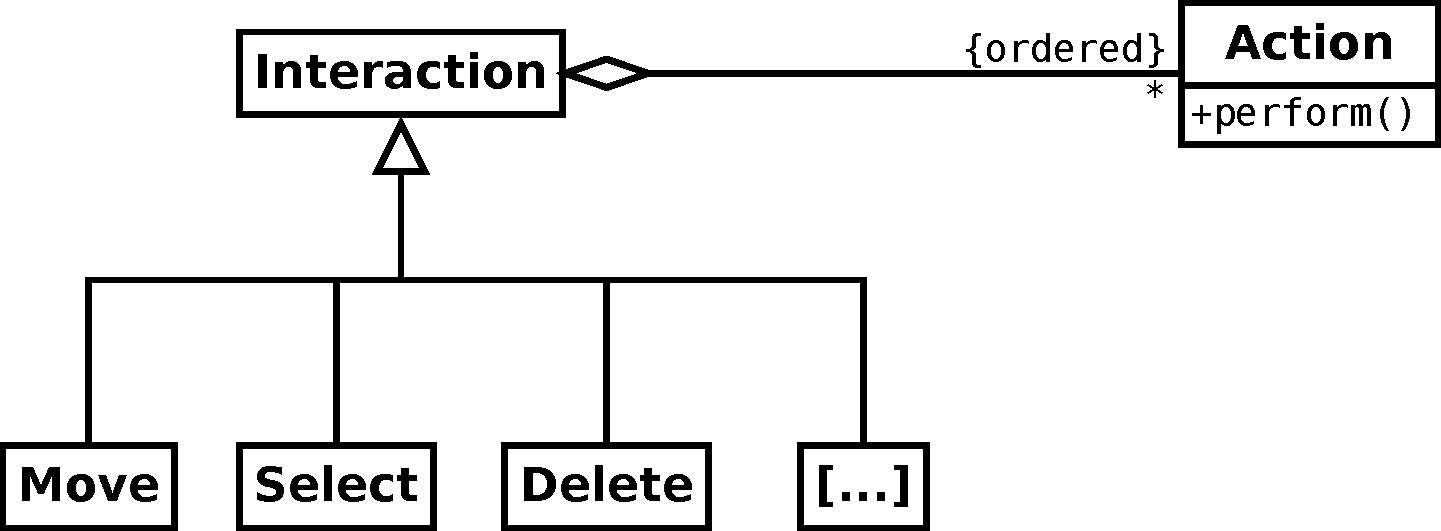
\includegraphics[width=\textwidth]{diagrams/action_interaction_simple.pdf}
    \caption[Relation between Interaction and Action (UML class diagram)]
    {Relation between Interaction and Action (UML class diagram)}
    \label{action_interaction_simple}
\end{figure}

Each interaction consists of one or more actions. Actions are tinier than
interactions and represent simple actions a user can execute. Interactions are
on a higher level of abstraction, they aggregate one or more actions to a
higher unit. An example for an action could be ``mouse down'' and this could be
part of the interaction ``move object''.

On another meta level, actions are events. To be more specific, events are
actions which occur on a fixed time. The time stamp is important to order the
events. Two different interactions can consist of the same set of actions, but
their order makes the difference. Figure \ref{action_interaction_complex}
shows the model on two different meta levels, where ``Event'' is an instance of
``Action'' and in table \ref{table:sequence} an exemplary sequence of events is
presented. The events in table \ref{table:sequence} are numbered in the order they
occurred.

\begin{figure}
    \centering
    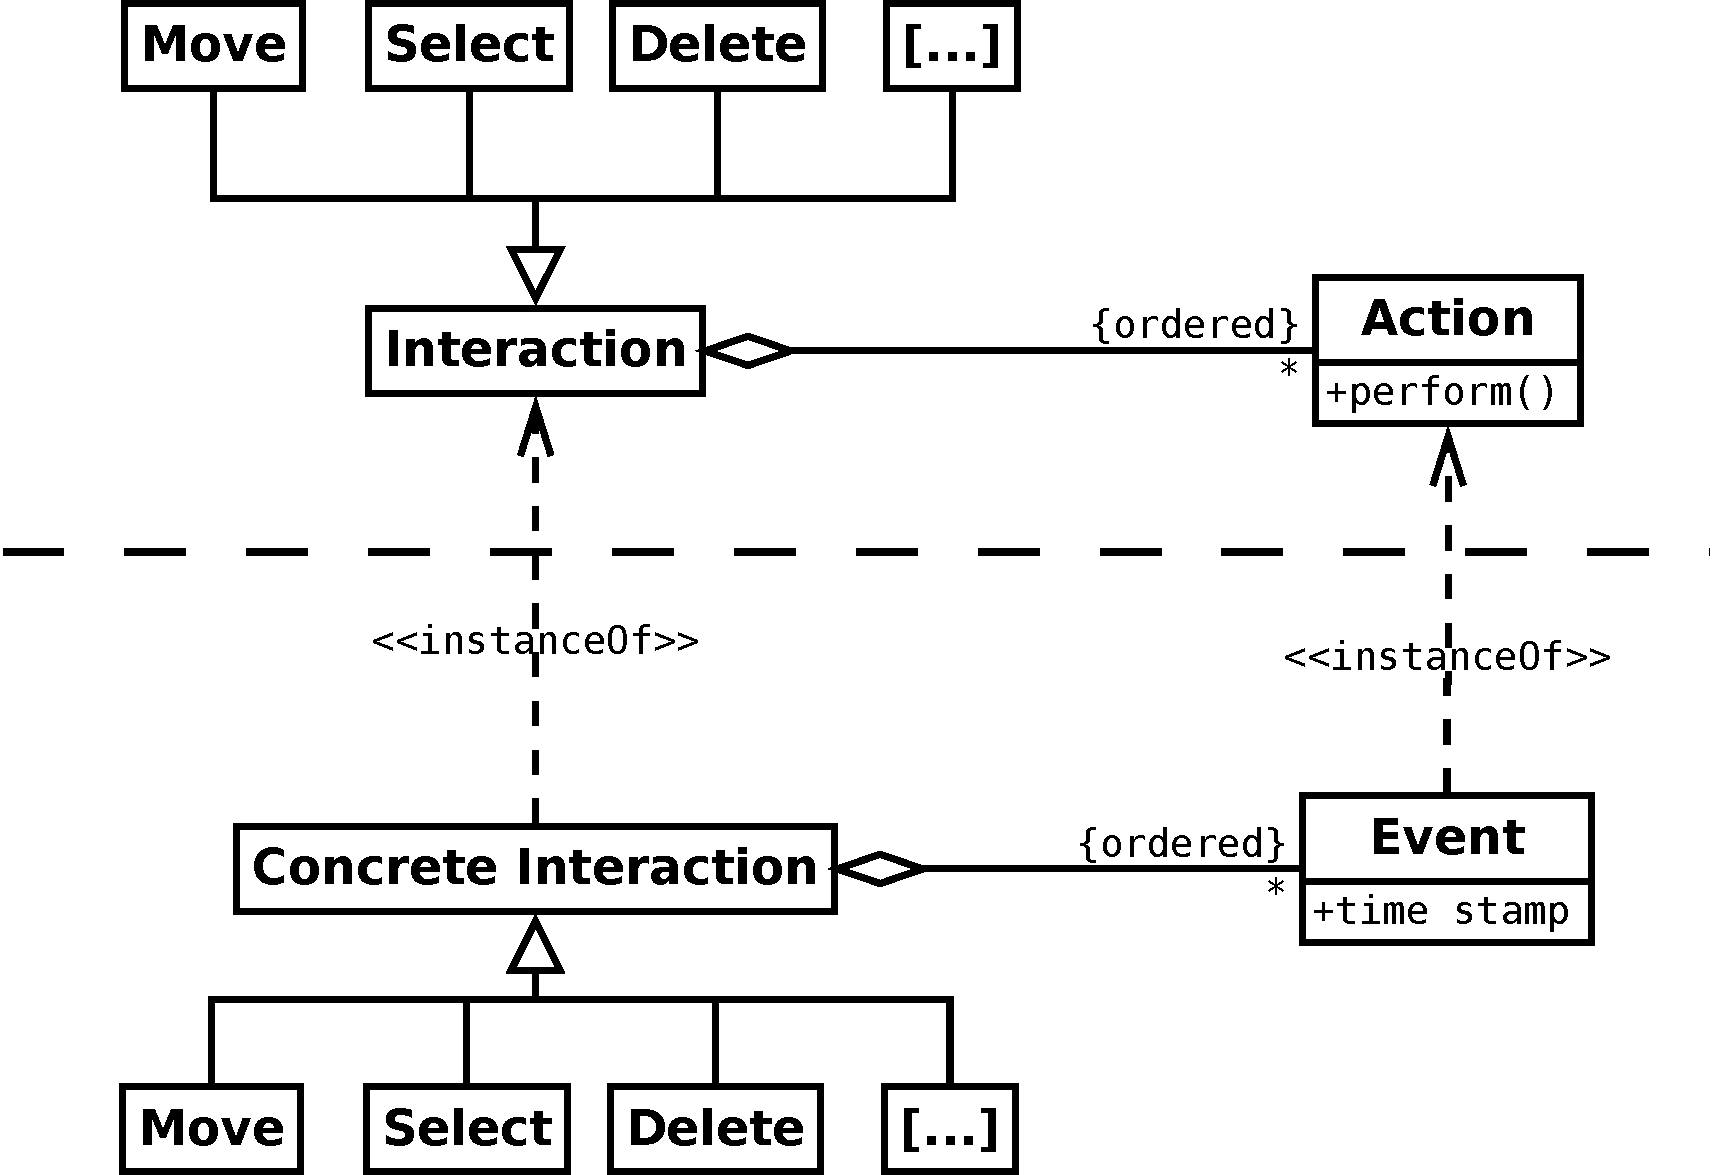
\includegraphics[width=\textwidth]{diagrams/action_interaction_complex.pdf}
    \caption[Different meta levels of Action and Interaction (UML class diagram)]
    {Different meta levels of Action and Interaction (UML class diagram)}
    \label{action_interaction_complex}
\end{figure}

\begin{table}
\caption[An Exemplary Sequence of Events]
{An Exemplary Sequence of Events}
\centering
\begin{tabular}{|r|c|l|}
    \hline
    Event & Action & Interaction \\ \hline
    [...] & [...] & [...] \\
    \hline \hline
    e15 & MouseDown & \multirow{3}{*}{Move} \\
    e16 & MouseMove & \\
    e17 & MouseUp & \\
    \hline \hline
    e18 & MouseDown & \multirow{2}{*}{Select} \\
    e19 & MouseUp & \\
    \hline \hline
    e20 & DELPress & Delete \\
    \hline \hline
    [...] & [...] & [...] \\ \hline
    \hline
\end{tabular}
\label{table:sequence}
\end{table}

At this point, activities need to be introduced. Activities are a way to
structure the game flow, even in non-linear games. Everything a student does
in the game can be associated to an activity. Activities are an abstract
concept, which group interactions to form a higher unit. This group building
is important to understand where a learner is in the learning process and
whether they are still efficiently learning or not. To explain this further, an
example will help: Blanchard (\cite{Blanchard2004b, Blanchard2009}) proposes
a game which models the work day of a
doctor in a hospital. The player can click on objects and gather information
about various instruments and methods of a doctor. If the game ``thinks'' that the learner is
not actually learning any more but only wandering around without scope, it
confronts the learner with a scenario (in Blanchard's case an accident
happened and the player has to conduct diagnoses) \cite{Blanchard2004b}. In
Blanchard's example, there are various activities a learner can perform and
these activities determine the way the game interacts with the player: if the
player is exploring the virtual world and learning stuff on its own, there is
no need to make up a scenario to bring them back on track. Figure
\ref{activity_motivation} shows the
relation between activities in the game and motivation. A more detailed
overview of some possible motivational factors is shown in figure
\ref{motivation}.

\begin{figure}
    \centering
    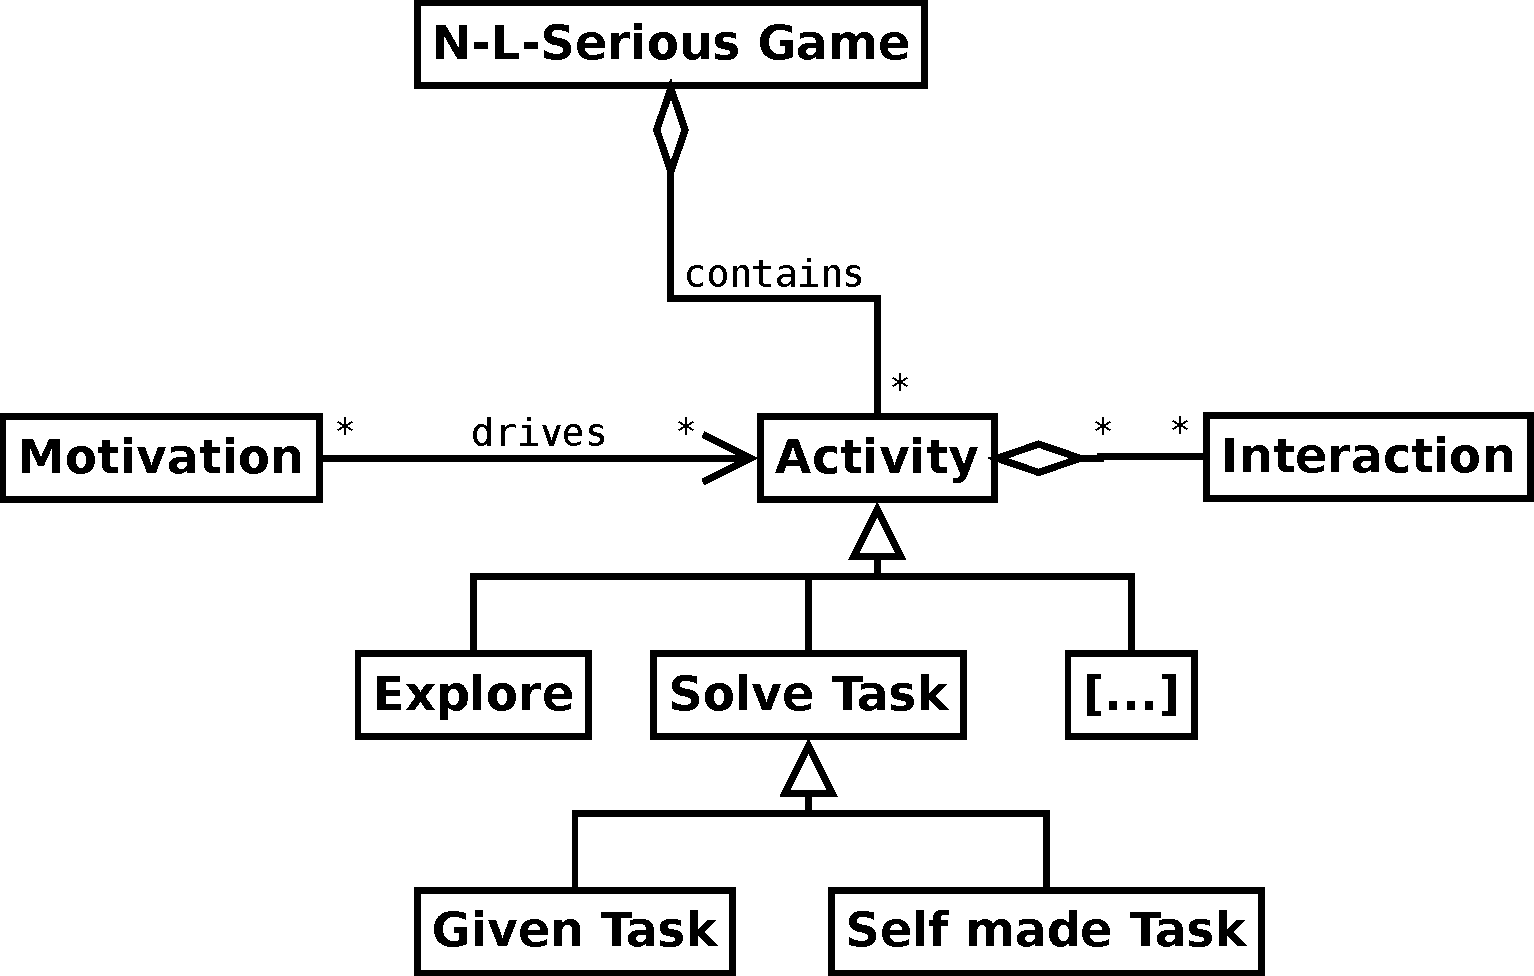
\includegraphics[width=\textwidth]{diagrams/activity_motivation.pdf}
    \caption[Different Activities in a Non-Linear-Serious Game (UML class diagram)]
    {Different Activities in a Non-Linear-Serious Game (UML class diagram)}
    \label{activity_motivation}
\end{figure}

\begin{figure}
    \centering
    \includegraphics[width=\textwidth]{diagrams/motivation.pdf}
    \caption[Motivational Factors (UML class diagram)]
    {Motivational Factors (UML class diagram)}
    \label{motivation}
\end{figure}

%~The game itself can be structured into activities. Activities are one level
%~higher than interactions. The whole learning experience can be covered with
%~activities. During each activity several interactions can be performed.

%~The goal of the framework is to monitor the actions of the player closely and draw
%~the consequences according to these actions. The actions of a user are the only characteristics we can
%~monitor directly. Of course there are physical features like heart rate, facial
%~expressions and others, but those cannot be monitored easily. Affection
%~detection in real-time, without human intervention is not an easy task
%~\cite{BLANCHARDb}. The most
%~promising methods go in the direction of face recognition, because new
%~computers often have a built-in camera to enable video-telephony and no
%~additional hardware is needed \cite{BLANCHARDb}.

%~Interactions are the very strong indicators of human behavior and if we
%~succeed to understand human behavior by monitoring the actions this would be a
%~very big step in the direction of intelligent learning systems. Anyways this
%~is still a theory and extensive studies are needed to prove whether it is
%~possible to understand behavior only from the actions or not.

\section{Problem Detection}
\label{Problem Detection}
In education it is important to react when a learner has a problem. Some
problems are simply too complex for a student to be resolved by themselves. These
problems have to be eliminated, otherwise the motivation of the student drops to
zero and changes to frustration. At some degree, problems can have a positive
effect on the learner and cause better problem solving skills, but not if they
are too complex to resolve.

The question is: what would a human tutor do, if they would watch closely
what the student is doing. A human tutor would categorize the problem and
depending on the situation they would support the learner or give them the chance
to solve the problem alone. This decision is very complex and depends on many
different factors. Some of which are the emotional state, learning history,
current knowledge, current activity and personality aspects of the learner. All this information
helps a human tutor to decide if an intervention is needed or not. Figure
\ref{problem_detection_process} shows the process of problem detection as a
human tutor would perform it.

\begin{figure}
    \centering
    \includegraphics[width=\textwidth]{diagrams/problem_detection_process.pdf}
    \caption[The Process of Problem Detection (UML activity diagram)]
    {The Process of Problem Detection (UML activity diagram)}
    \label{problem_detection_process}
\end{figure}

%~Figure \ref{problem_type_support} shows some
%~of the most determinant factors.

%~\begin{figure}
    %~\centering
    %~\includegraphics[width=\textwidth]{diagrams/problem_type_support.pdf}
    %~\caption[The Problem Type determines the Support]
    %~{The Problem Type determines the Support}
    %~\label{problem_type_support}
%~\end{figure}

But what exactly is a problem? How can we humans decide what a problem is
and can a machine do the same? We humans detect problems because we have
certain expectations. Expectations are a sort of mental schemes which are
represented in our brain. When a student fulfills our expectations,
everything is fine. But if the student fails to fulfill the expectations, we
have two possibilities: we can adapt our scheme because the student found
another solution for the task or we can correct the student and guide them in
the right direction, hence support the student. The big question is: can
machines do that? Of course they can, we just need to find an appropriate
description of expectation and a measure to assess the state of the learner
which can be matched to the expectation.

As shown in figure \ref{system_problem_support} on page
\pageref{system_problem_support}, the problem can be
categorized into three big categories: motivational problems, comprehension
problems (content-related) and problems which regard the usage of the software
itself. Categorizing the problem is important to decide which way of support
is the best to resolve the problem.

\section{Supporting the Learner}
\label{Supporting the learner}
Support is easy, some may think, but thats not the case! Dumb support may be
easy, but supporting the learner in a smart way is a very ambitious task.
Smart support needs to understand the learner and act in respect to their
problems and preferences. In order to do that, a dynamic system needs to be
build, a system that can react to changes which definitely occur during the
process of learning.

The support should follow pedagogic principles developed over many years.
Simple forms of support (some are shown in figure \ref{system_problem_support} on
page \pageref{system_problem_support}) are: providing additional facts, repeat a lesson,
highlight tools needed to complete a task, show another description of the
task to foster a better understanding of the task. More complex forms of
support could be something like scaffolding: the learner gets a complex task,
too complex for them to solve alone, but the difficulty makes it more
interesting than a easy and dumb task. At the beginning the system supports
the learner and takes over some parts of the task. After some time, the support
(scaffold) is reduced bit by bit until the learner is capable to carry out all
subtasks alone. Scaffolding has been used in some computer based instruction
systems and first results are very promising \cite{Azevedo2005c,
ElSaadawi2010, Lai2009a}. Scaffolding could be one
of the pedagogic strategies of an ``intelligent support system''.

\section{Pedagogical Agents}
\label{pedagogical_agents}
Pedagogical Agents are pieces of software which concentrate on the interaction
between the user and the system. They provide a life-like interface which
gives feedback and can be triggered to answer questions or carry out some
tasks for the user. The most famous (pedagogical) agent probably is the
Microsoft Paper Clip, which was one of the first attempts to develop a
pedagogical agent for Microsoft Office. Although the Paper Clip did not seem very intelligent, the
research which was conducted back then was very important. Todays pedagogical
agents are far more advanced, an example for such an agent is ``Herman the
Bug'' (see figure \ref{herman_the_bug}), which supports the learner in
the game ``Design-A-Plant'' \cite{Lester1997c}.

\begin{figure}[t]
    \centering
    \includegraphics[width=\textwidth]{images/pedagogical_agent.jpeg}
    \caption[Herman the Bug, a Pedagogical Agent]
    {Herman the Bug, a Pedagogical Agent \cite{Lester1997c}}
    \label{herman_the_bug}
\end{figure}

Such pedagogical agents are used in learning software to keep the learner on track and
motivated during the learning process. Many studies have been conducted about
the way such agents should look like, interact with the learner and how they
improve learning: \cite{Nunes2002b, Conati2004b, Johnson2000, Slater2000a,
Baylor2003b, Blanchard2004b, Voerman1997a}, etc. One of the
most promising studies was conducted by Moreno et al., where they tested the
hypothesis if pedagogical agents can ``promote constructivist learning in a
discovery-based learning environment'' \cite{Moreno2000a}. The study of Moreno
et al. \cite{Moreno2000a} also examines the influence of the agents' image,
voice and language style on a deeper learning experience.

There is no need to go in more detail here, because there are many solutions for
pedagogical agents out there which can be used. Nevertheless it should be emphasized,
how promising the results of pedagogical agents in e-Learning are:
Lester et al. conducted a large study to evaluate the effectiveness of
pedagogical agents and came to the conclusion that pedagogical agents decrease
the problem related errors of students during complex tasks significantly
\cite{Lester1997a}. Another study shows significant increases in the problem
solving skills, when a pedagogical agent is used \cite{Lester1997c}.

\begin{figure}
    \centering
    \includegraphics[height=\textheight]{diagrams/system_problem_support_portrait.pdf}
    \caption[System Overview including Problem and Support (UML class diagram)]
    {System Overview including Problem and Support (UML class diagram)}
    \label{system_problem_support}
\end{figure}
